\documentclass[]{article}

\usepackage{graphicx}
\usepackage{Bookmark}

%opening
\title{Testing Document}
\author{Grant Louat}

\begin{document}

\maketitle

\begin{abstract}
This document details the testing of all functions, and their current state. Each function will be tested in isolation. This document should detail by what criteria the function has been deemed correct, the date and who did the testing. It should also have a listing of the working code so there is no confusion over different versions. This will quickly tell everyone which functions have been confirmed correct, and the rigour to which that assertion was made. It will also tell them when it was confirmed in case they have been working on a local copy of the code, and who deemed it correct in case they have questions. This document should also have a description of the function so that people know what the function should be doing when it is working.\newline
The document deals only with the isolation testing of each function. The functions will also need to be tested in an integration phase later. \newline
WARNING: DO NOT INCLUDE ANYTHING IN THIS DOCUMENT UNLESS YOU ARE CERTAIN THAT IT IS COMPLETELY ERROR FREE! \newline Even if it is a simple one line function there could be a type issue or something. Anything document will be assumed working, and if a single error remains it will nullify the entire document. If a function is too large or complex to test and verify in complete certainty then it should be split into smaller functions to solve parts of the problem. Make sure also to include WHY you verified the function correct, as your rigour may not meet the standard of someone else's.
\end{abstract}

\newpage
\section{Common:}

\subsection{DIV\_X:}
\subsubsection{Status:}
Working as of 11:30 25/9/2014 - Grant

\subsubsection{Description:}
This set of Macros are designed to divide an integer by a power of two.

\subsubsection{Criteria:}
The value of 1024 was tested for each of the macros, and due to the simplicity and nature of the macros no other values need be tested.

\subsubsection{Working code:}
\#define DIV\_2(v) ((v) $>>$ 1)       //Divide by 2

\newpage
\section{Temperature Module:}

\subsection{ReadTempx2:}

\subsubsection{Status:}
Currently untested as of 8am 26/9/14 - Grant

\subsubsection{Description:}
Returns the temperature (x2) in degrees Celsius by performing an A/D conversion on the analogue output from the temperature sensor.

\subsection{ReadTemp:}
\subsubsection{Status:}
Working as of 8am 26/9/2014 - Grant

\subsubsection{Criteria:}
This function was tested in isolation of the ReadTempx2, and the assertion only applies to this function. A ReadTempx2 stub function was written to simply return the value of 40 to test the ReadTemp function.

\subsubsection{Description:}
The function simply calls the ReadTempx2 function and divides the result by 2.

\subsubsection{Working Code:}
unsigned char readTemp(void)
{
	unsigned char temp;
	
	temp = readTempx2();
	
	return DIV\_2(temp);
}

\subsection{RawTemp:}

\subsubsection{Status:}
Working as of 8:30am 26/9/2014 - Grant

\subsubsection{Criteria:}
The function was tested in isolation of the ReadTemp functions. A dummy function placed the value of 60 into the lastTempx2 variable, and the RawTemp function worked as described.

\subsubsection{Description:}
This function returns the uncalibrated result of the last temperature read. E.g. the raw sensor output. A temperature read is performed by either a ReadTemp or ReadTempx2 call. \newline:
This function cannot be completely tested in isolation as it requires an external static declaration of the lastTempx2 variable. It also requires the ReadTemp and ReadTempx2 functions to write to this variable when they perform a read.

\subsubsection{Working Code:}
unsigned char rawTemp(void)
{
	return DIV\_2(lastTempx2);
} 

\subsection{Calibrate Temp:}
\subsubsection{Status:}
Working as of 10:30am 26/9/2014 - Grant

\subsubsection{Description:}
Calibrates the last temperature read to the passed reference value by updating a static variable.

\subsubsection{Criteria:}
This function was tested in isolation of the readTemp functions. a dummy readTempx2 function which just returned 15deg (and set the static variable) was written, and the calibration function called to calibrate it to 20 deg, and then 10 deg. In both cases a second call of readTempx2 returned the desired value even though the 'raw data' was simply hard coded in.

\subsubsection{Working Code:}
void calibrateTemp(unsigned char reference)
{
	calibration\_offset = 2 * (reference - DIV\_2(lastTempx2));
}

\subsection{GetTemp:}

\subsubsection{Status:}
Working as of 10:30 26/9/2014 - Grant

\subsubsection{Description:}
Returns the result of the last temperature read.

\subsubsection{Criteria:}
This is just an accessor function, so it simply returns the value of a static variable.

\newpage
\section{Range}

\subsection{SPD\_SND Macro}
\subsubsection{Status:}
Working as of 10:30 25/9/14 - Grant

\subsubsection{Description:}
This macro uses integer operations, so merely approximates the actual value to avoid lengthy floating point operations. 

\subsubsection{Criteria:}
Each temperature from 0 to 100 deg C was tested and compared to the actual formula result. There is some deviation due to the exclusive use of integer operations, but negligible See Fig. \ref{fig:SND_comp}.\newline 

\subsubsection{Working Code:}
\#define SPD\_SND(T) (DIV\_128(332 * (unsigned int)sqrt(16384 + T * (unsigned int)60)))

\begin{figure}
	\centering
	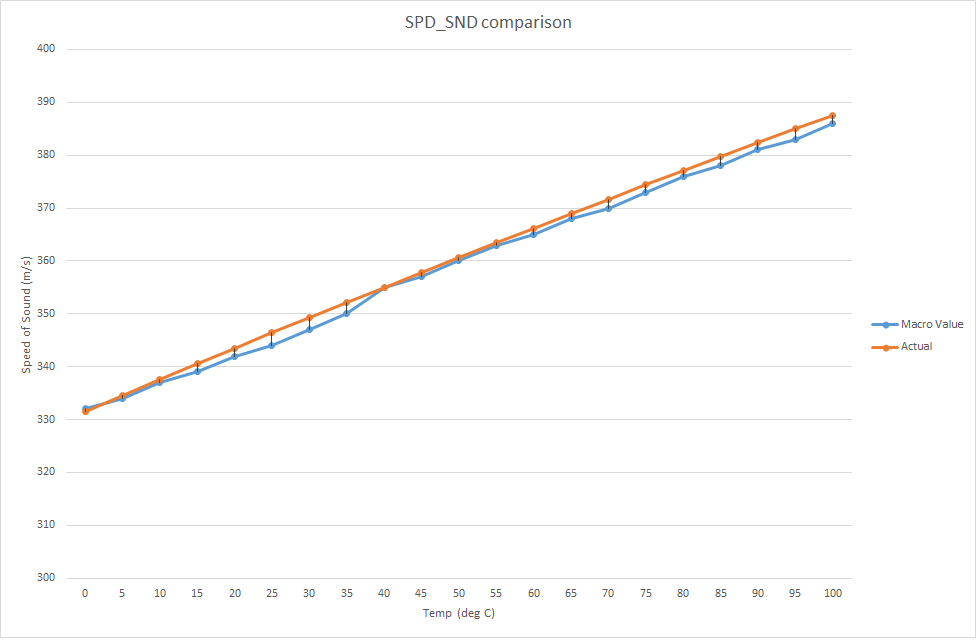
\includegraphics[width=0.7\linewidth]{SND_comp}
	\caption{Comparison between SPD\_SND() Macro output and actual function value}
	\label{fig:SND_comp}
\end{figure}

\subsection{calibrateRange:}
\subsubsection{Status:}

\subsubsection{Description:}

\subsubsection{Criteria:}

\subsubsection{Working Code:}

\subsection{rawRange:}
\subsubsection{Status:}
untested as of 11am 26/9/2014 - Grant

\subsubsection{Description:}
Accessor function - simply returns the uncalibrated sensor output from the last range calculation.

\subsubsection{Criteria:}

\subsection{range:}
\subsubsection{Status:}
Untested as of 11am 26/9/14 - Grant

\subsubsection{Description:}
This function performs a read of both the ultrasonic and IR sensors, fuses them and calibrates the result. The current version simply averages the IR and ultrasonic ranges as an initial fusion method.

\subsubsection{Criteria:}

\subsection{rangeIR:}
\subsubsection{Status:}
Untested as of 11am 26/9/14 - Grant

\subsubsection{Description:}
This function performs a read of the IR sensor, calibrates it and returns the result.

\subsubsection{Criteria:}

\subsection{rangeUS:}
\subsubsection{Status:}
Untested as of 11am 26/9/2014 - Grant

\subsubsection{Description:}
This function performs a read of the Ultrasonic sensor (if not already started), calibrates it and returns the result.

\subsection{ConfigureRange:}
\subsubsection{Status:}
Untested as of 12pm 26/9/14

\subsubsection{Description:}
This function configures everything needed in the Range module to begin sampling the range.

\subsubsection{Criteria:}

\subsection{BeginUS:}
\subsubsection{Status:}
Untested as of 12pm 26/9/2014

\subsubsection{Description:}
This function begins an ultrasonic scan and returns. The returning echo will be serviced by an interrupt and the value will be stored in the range module for the next rangeUS call.

\subsection{rangeISR:}
\subsubsection{Status:}
Untested as of 12pm 26/9/2014 - Grant

\subsubsection{Description:}
This function acts as the service routine for the range module. The exact function will depend on the implementation of the range module and what interrupts are used.

\subsubsection{Criteria:}

\newpage
\section{Tracking}

\subsection{ConfigureBase:}
\subsubsection{Status:}
Currently incomplete and untested as of 12:15pm 26/9/2014 - Grant

\subsubsection{Description:}
This function configures the pan tilt mechanism (which is acting as the base) so that it is ready for initial use.

\subsubsection{Criteria:}

\subsection{Search:}
\subsubsection{Status:}
Currently incomplete and untested as of 12:15pm 26/9/2014 - Grant

\subsubsection{Description:}
This function increments the pan tilt mechanism in a search pattern.

\subsubsection{Criteria:}

\subsection{trackingISR:}
\subsubsection{Status:}
Untested as of 1:20pm 26/9/2014 - Grant

\subsubsection{Description:}
This function acts as the ISR for the tracking module. The exact functionality will depend on what interrupts are associated with the tracking module, and how they are implemented.

\subsubsection{Criteria:}


\subsection{Edge:}
\subsubsection{Status:}
Currently untested as of 1:20pm 26/9/2014

\subsubsection{Description:}
This function finds the edge of the target in both the azimuth and declination degrees of freedom, and uses that to find (and track) the centre of the target. It could also be used as a rudimentary target verification based on the approximate size of the target.

\subsubsection{Criteria:}


\subsection{moveBase:}
\subsubsection{Status:}
Currently incomplete and untested as of 1:20pm 26/9/2014 - Grant

\subsubsection{Description:} 
This function will move the pan tilt mechanism to the given inclination and declination.

\subsubsection{Criteria:}

\subsection{Validate:}
\subsubsection{Status:}
Currently working as of 1:30pm 26/9/2014 - Grant

\subsubsection{Description:}
This function validates a given delay to ensure that it is between 1000ms and 2000ms, coercing it if not.

\subsubsection{Criteria:}
This function was tested by passing it values of 100, 1500 and 10000, which includes one of each possible case. In each case the function responded appropriately and gave the desired response.

\subsubsection{Working Code:}
void validate(unsigned int *delay)
{
	if (*delay < 1000)
	{
		*delay = 1000;
	}
	if (*delay > 2000)
	{
		*delay = 2000;
	}
}

\subsection{direction2Delay:}
\subsubsection{Status:}
Currently incomplete and untested as of 1:30pm 26/9/2014

\subsubsection{Description:}
This function converts a desired direction into a pwm delay format that can then be used to generate the appropriate pwm.

\subsubsection{Criteria:}

\newpage
\subsection{Push Macro:}
\subsubsection{Status:}
Working as of 1:45pm 26/9/2014 - Grant

\subsubsection{Description:}
This macro pushes a byte onto a circular buffer. If the buffer is full then it begins overwriting the first data in the buffer.

\subsubsection{Criteria:}
This macro has been tested by pushing a byte onto an empty buffer, a partially filled buffer and a completely filled buffer. In each case the result was as documented.

\subsubsection{Working code:}
\#define push(byte, buf) buf.data[buf.head] = byte; if(full(buf)) incMod(buf.tail); incMod(buf.head)

\subsection{Pop Macro:}
\subsubsection{Criteria:}
Working as of 2:00pm 26/9/2014 - Grant

\subsubsection{Description:}
This macro pops a byte from a circular buffer. If the buffer is empty it returns whatever is in the first element location and does not change the pointers.

\subsubsection{Criteria:}
This macro has been tested with both empty and non-empty buffers and in each case it functions as documented.

\subsubsection{Working Code:}
\#define pop(buf) buf.data[buf.tail]; if (!empty(buf)) incMod(buf.tail)

\subsection{Init Macro:}
\subsubsection{Status:}
Working as of 2pm 26/9/2014 - Grant

\subsubsection{Description:}
This macro initialises a buffer before it can be used - It initializes the pointers to zero. This function will also completely clear a circular buffer.

\subsubsection{Criteria:}
This macro was tested by simply operating on a circularBuffer which was not previously initialized and making sure that it was subsequently initialised.

\subsubsection{Working Code:}
\#define init(buf) buf.head = 0; buf.tail = 0

\subsection{Peek Macro:}
\subsubsection{Status:}
Working as of 2:05pm 26/9/2014 - Grant

\subsubsection{Description:}
This macro returns the next byte that will be popped off the buffer, without removing that element from the buffer. If the buffer is empty it will simply return whatever happens to be in the first element.

\subsubsection{Criteria:}
This macro was tested by simply operating on a macro several times (between which push and pop operations were implemented) and making sure the correct thing was returned.

\subsubsection{Working Code:}
\#define peek(buf) buf.data[buf.tail]

\subsection{Full Macro:}
\subsubsection{Status:}
Working as of 2:05pm 26/9/2014 - Grant

\subsubsection{Description:}
This macro returns non-zero is the buffer is full, and zero otherwise.

\subsubsection{Criteria:}
This macro was tested by operating on a number of circular buffers, both full and not full (including empty), and in each case it returned the correct thing.

\subsubsection{Working Code:}
\#define full(buf) (buf.tail == (buf.head + 1) \% BUFFERLENGTH)

\subsection{Empty:}
\subsubsection{Status:}
Working as of 2:10pm 26/9/2014 - Grant

\subsubsection{Description:}
This macro returns non-zero if the buffer is empty. Otherwise it returns zero.

\subsubsection{Criteria:}
This macro was tested on both empty and non-empty buffers, including full buffers. In all cases the macro returned the expected result.

\subsubsection{Working Code:}
\#define empty(buf) (buf.head == buf.tail)

\subsection{IncMod Macro:}
\subsubsection{Status:}
Working as of 2:30pm 26/9/2014 - Grant

\subsubsection{Description:}
This macro increments a buffer pointer and takes the modulus with the buffer length (defined by BUFFERLENGTH), which will loop back to zero, making the buffer circular.

\subsubsection{Criteria:}
This macro has been tested with a range of values from 0 to BUFFERLENGTH. In each case the macro returned the response as documented.

\subsubsection{Working Code:}
\#define incMod(ptr) (ptr = ++ptr \% BUFFERLENGTH)

\subsection{ConfigureSerial:}
\subsubsection{Status:}
Untested as of 2:45pm 26/9/2014 - Grant

\subsubsection{Description:}
This function sets up and configures the serial UART for communication to the remote terminal.

\subsubsection{Criteria:}

\subsection{Transmit:}
\subsubsection{Status:}
Untested as of 2:50pm 26/9/2014 - Grant

\subsubsection{Description:}
This function pushes a string onto the serial transmit buffer and enables the transmit interrupt to begin transmitting the buffer (if not already transmitting).

\subsubsection{Criteria:}

\subsection{receiveEmpty:}
\subsubsection{Status:}
Working as of 2:50pm 26/9/2014 - Grant

\subsubsection{Description:}
This function returns non-zero if the receive buffer is empty. Otherwise it returns 0.

\subsubsection{Criteria:}
This function was tested in isolation by creating a circular buffer and calling the function between push and pop actions to test empty, non-empty and full cases. In each case the the function returned the expected result.

\subsubsection{Working Code:}
char receiveEmpty(void)
{
	return empty(receive\_buffer);
}


\subsection{receivePeek}
\subsubsection{Status:}
Working as of 2:55pm 26/9/2014 - Grant

\subsubsection{Description:}
This function applies the peek macro to the receive buffer and returns the result.

\subsubsection{Criteria:}
The function was tested in isolation on a circular buffer in full, empty and non-empty cases, and each time the function returned the correct result.

\subsubsection{Working Code:}
char receivePeek(void)
{
	return peek(receive\_buffer);
}

\subsection{receivePop:}
\subsubsection{Status:}
Working as of 3pm 26/9/2014 - Grant

\subsubsection{Description:}
This function applies the pop macro to the receive buffer and returns the result.

\subsubsection{Criteria:}
The function was tested in isolation on a circular buffer in full, empty and non-empty cases. Each time the result was as outlined in the documentation.

\subsubsection{Working Code:}
char receivePop(void)
{
	return pop(receive\_buffer);
}

\subsection{serialISR:}
\subsubsection{Status:}
Untested as of 3:10pm 26/9/2014 - Grant

\subsubsection{Description:}
This function acts as the interrupt service routine for the serial module. The primary purpose will be to handle the receive and transmit interrupts.

\subsubsection{Criteria:}

\newpage



\end{document}
